\chapter{Approach}
\label{ch:approach}
%%%%%%%%%%%%%%%%%%%%%%%
% - description of the designed system
% - analysis and review of the current software architecture
%%%%%%%%%%%%%%%%%%%%%%%

In this chapter we give an overview of the current software architecture on which the Basilisk platform is build.

The basic architecture pattern of the Basilisk platform is the microservice architecture (see chapter \ref{sec:microservice_architecture} for a short description). 
This means that the platform is divided into multiple services which can run on different hardware systems and interact with each other via a message queue system.
\\


Figure \ref{fig:basilisk_high_level_design} gives an overview of the microservice architecture for the Basilisk framework and the most important messages send between the services.
\begin{figure}[tbph]
	\centering
	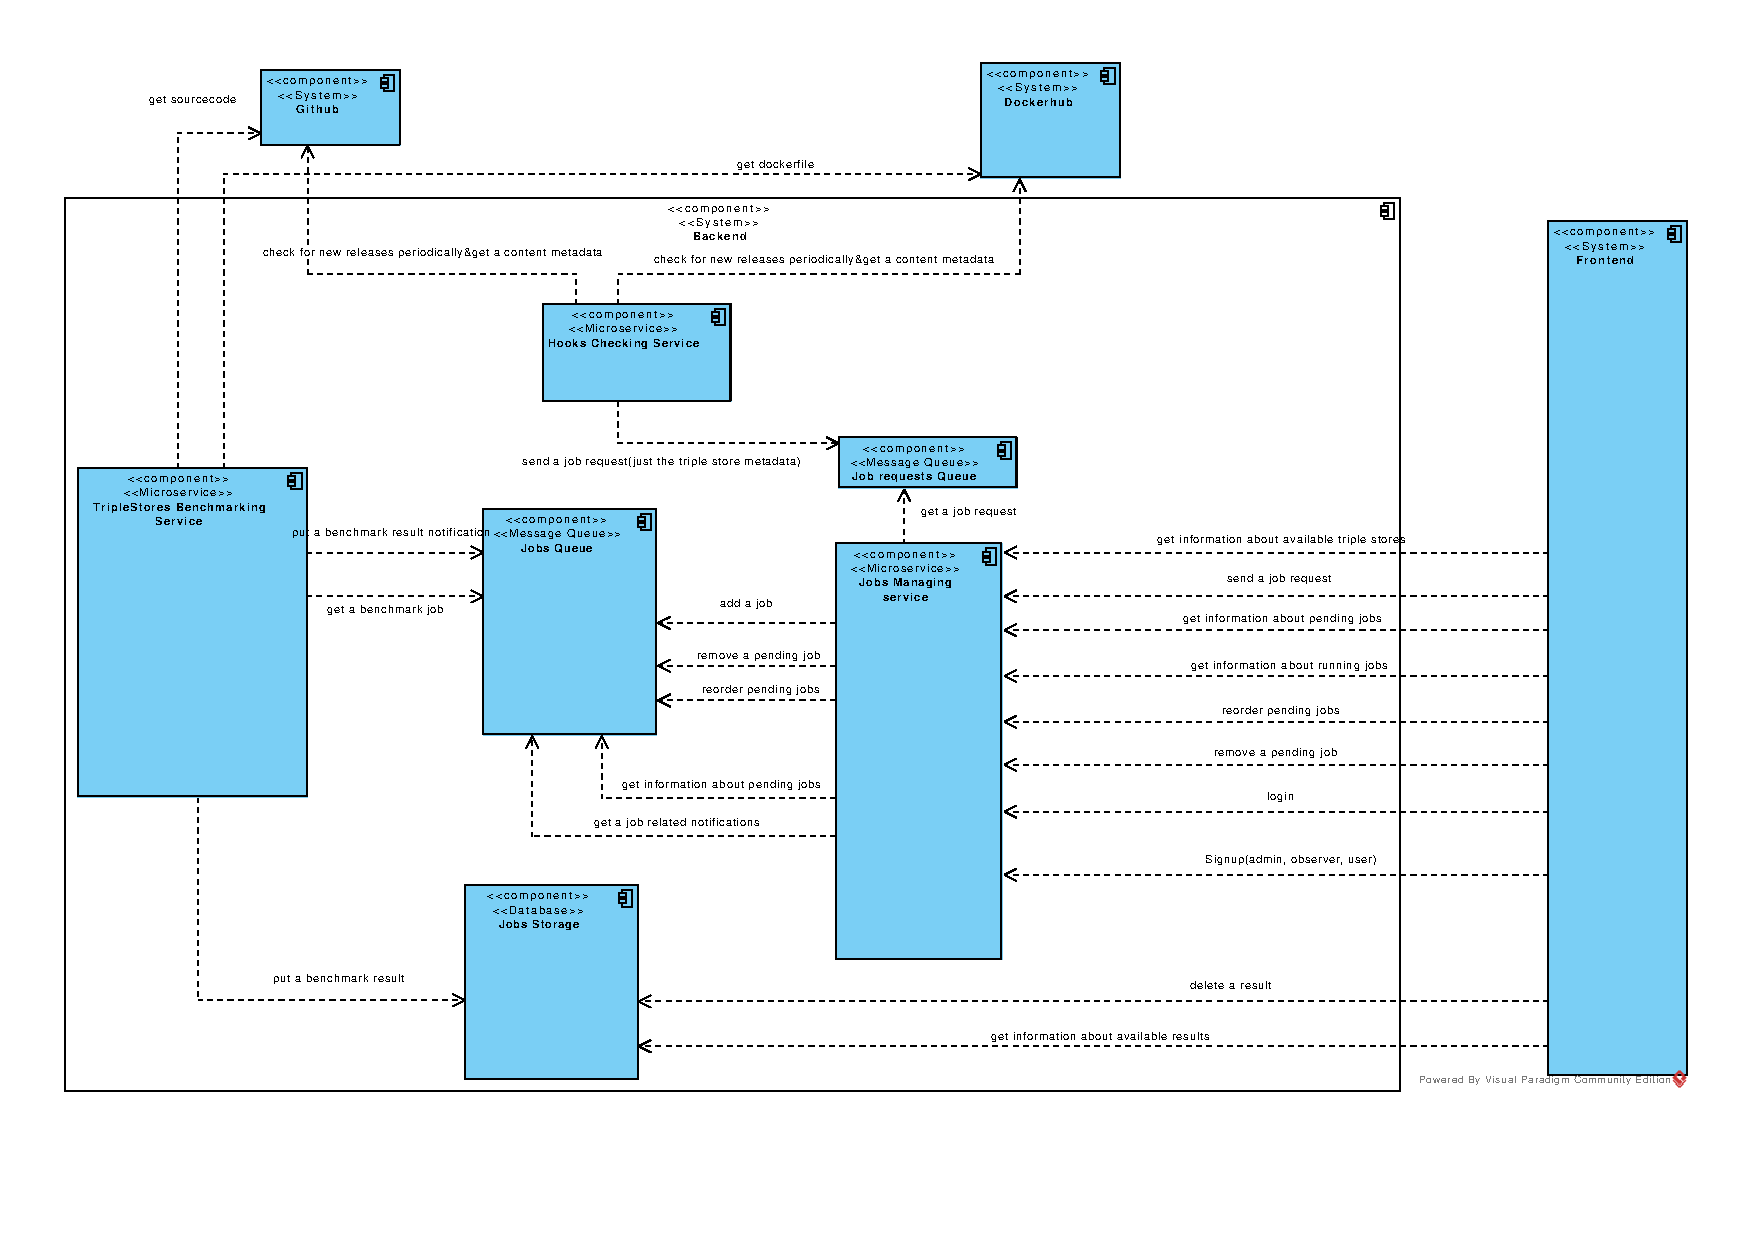
\includegraphics[width=1.1\textwidth]{figures/basilisk_high_level_design.pdf}
	\caption{High level design of the Basilisk framework}
	\label{fig:basilisk_high_level_design}
\end{figure}
\\

The next sections explain the three main services, namely Hooks Checking Service (\ref{sec:hooks_checking_service}), Jobs Managing Service (\ref{sec:jobs_managing_service}), and \ts{} Benchmarking Service (\ref{sec:ts_benchmarking_service}).

\section{Hooks Checking Service}
\label{sec:hooks_checking_service}
The main task of the hooks checking service is to observe Github and Dockerhub repositories for new releases or changes.


\section{Jobs Managing Service}
\label{sec:jobs_managing_service}
The Jobs Managing Service processes the requests coming from the web-frontend, checks if the Hooks Checking Service has found a new version for a benchmark and creates jobs for new benchmarks.


\section{\ts{} Benchmarking Service}
\label{sec:ts_benchmarking_service}
Lastly the \ts{} Benchmarking Service executes the benchmarks given to it and saves the results to a database.